\documentclass[12pt,a4paper]{scrartcl}
\usepackage[utf8]{inputenc}
\usepackage[english,russian]{babel}
\usepackage{indentfirst}
\usepackage{misccorr}
\usepackage{graphicx}
\usepackage{amsmath}
\usepackage{multirow}
\usepackage{pgfplots}
\usepackage{slashbox}
\usepackage[top=1cm, bottom=1cm, left=1cm, right=1cm]{geometry}
\pgfplotsset{compat=1.9}

\begin{document}
	\graphicspath{{C:/Users/Alex/OneDrive/Изображения/TexImgs}}
	
	\newcommand{\ms}{\mathstrut}
	\newcommand{\msp}{\hspace{0.5cm}}
	\newcommand{\al}{\alpha}
	\newcommand{\dg}{^\circ}
	\newcommand{\qd}[2]{^{\frac{#1}{#2}}}
	\newcommand{\qdm}[2]{^{-\frac{#1}{#2}}}
	\newcommand{\lm}[2]{\underset{#1 \rightarrow #2}{\lim}}
	\newcommand{\sfrac}[2]{\dfrac{\strut #1}{\strut #2}}
	\newcommand{\equal}[1]{\overset{(#1)}{=}}
	\newcommand{\linevdots}{\ \raisebox{-.08\height}{\vdots}\ }
	\newcommand{\linecvdots}{\ \raisebox{-.08\height}{\vdots}\hspace{-0.13cm}\raisebox{.15\height}{\cancel{\phantom{a}}\hspace{0.06cm}}}
	\newcommand{\combox}[1]{\ms \msp \msp \begin{minipage}{0.95\linewidth}
			#1
	\end{minipage}}
	
	\newtheorem{pr}{Задача}
	\newtheorem{ex}{Пример}
	\newtheorem{dfn}{Def}
	\newtheorem{theorem}{Th}
	
	\newenvironment{slv}{\ms \msp \textit{Решение:}}{}
	\newenvironment{proof}{\ms \msp \textit{Доказательство: }}{\hfill $\square$}
	
	\begin{titlepage}
		
		\vspace*{\fill}
		
		\begin{center}
			
\includegraphics[scale=0.8]{MIPT.png}
			\\[0.7cm]\Huge Московский Физико-Технический Институт\\(национальный исследовательский университет)
			\\[2cm]\LARGE Отчет по эксперименту
			\\[0.5cm]\noindent\rule{\textwidth}{1pt}
			\\\Huge\textbf{Определение вязкости жидкости\\по скорости истечения\\через капилляр}
			\\[-0.5cm]\noindent\rule{\textwidth}{1pt}
		\end{center}
		
		\begin{flushleft}
			\textit{Работа №2.2.5; дата: 14.02.22}\hfill\textit{Семестр: 2}
		\end{flushleft}
		
		\vspace*{\fill}
		
		\begin{flushleft}
			Выполнил: \hspace{\fill} Группа:
			\\Кошелев Александр \hspace{\fill} Б05-105
		\end{flushleft}
	\end{titlepage}
	
	%Страница 2
	
	\begin{flushleft}
		\footnotesize{Определение вязкости жидкости по скорости истечения через капилляр} \hspace{\fill} \footnotesize{2}
		\\[-0.3cm]\noindent\rule{\textwidth}{0.3pt}
	\end{flushleft}
	
	\section{Аннотация}
	
	В данной работе изучается влияние вязкости жидкости на ее ламинарное течение. При этом рассматривается истечение через капилляр и определяется вязкость воды. Также происходит знакомство с вискозиметром Оствальда и применение его на практике для измерения вязкости растворов глицерина разной концентрации.
	
	\textbf{Схема установки:}
	\begin{center}
		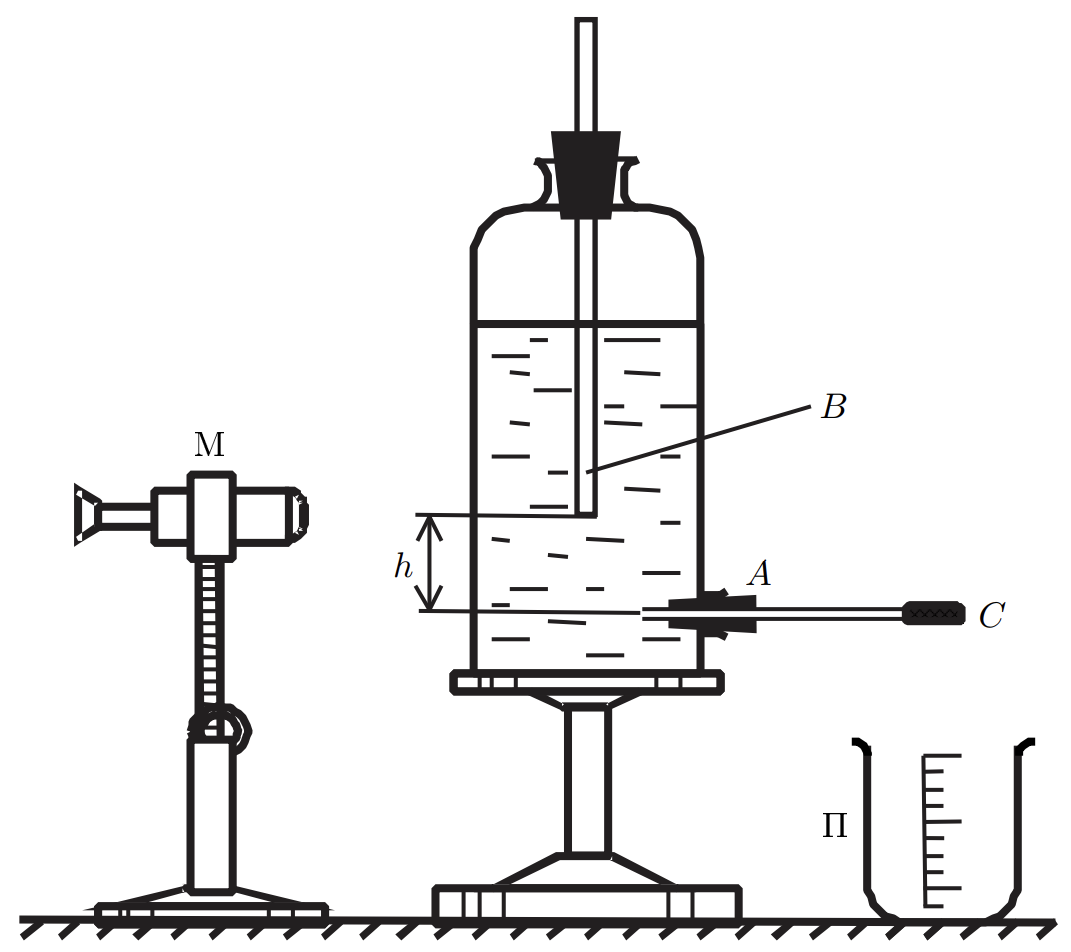
\includegraphics[scale=0.3]{PIC_1.png}
		\\\textbf{Рис. 1:} Схема установки А
	\end{center}
	
	
	\textbf{В работе используются:} пробка А с капилляром С, сосуд Мариотта, пробка с толстой трубкой В, микроскоп М на стойке, мензурка П, секундомер.
	
	\section{Теоретические сведения}
	
	Из курса общей физики известна формула Пуазейля:
	$$Q = \pi\sfrac{P_1 - P_2}{8\eta l}R^4$$
	
	Из нее следует, что вязкость жидкости $\eta$ можно определить, измеряя ее расход $Q$, перепад давления $P_1 - P_2$, длину капилляра $l$ и его радиус $R$. Также вспомним число Рейнолдса:
	$$Re = \sfrac{\upsilon R \rho}{\eta}$$
	
	Из предыдущих уравнений и уравнения Бернулли определяется применимость формулы Пуазейля. В нашем случае ламинарное течение устанавливается после расстояния $a$:
	$$a \approx 0.2 R \cdot Re$$
	
	То есть формула Пуазейля справедлива при длине капилляра $l \gg a$.
	
	%Страница 3
	
	\newpage
	
	\begin{flushleft}
		\footnotesize{Определение вязкости жидкости по скорости истечения через капилляр} \hspace{\fill} \footnotesize{3}
		\\[-0.3cm]\noindent\rule{\textwidth}{0.3pt}
	\end{flushleft}
	
	\section{Проведение эксперимента}
	
	\subsection{Определение вязкости воды}
	
	\paragraph{Измерение параметров установки} \hfill
	
	Занесем в таблицу длину $l$ капиллярной трубки и ее диаметр $d$.
	\begin{center}
		\begin{tabular}{|c|c|}
			\hline
			$l$, мм & $d$, мм \\\hline
			$135 \pm 1$ & $1.00 \pm 0.05$ \\\hline
		\end{tabular}
		\\\textbf{Табл. 1:} Параметры установки 
	\end{center} 

	\paragraph{Определение поправки для разницы давлений} \hfill
	
	\par Найдем высоту $\Delta h$, при которой поток жидкости остановится:
	$$\Delta h = (1.0 \pm 0.1)\ \text{см}$$
	
	\paragraph{Измерение расхода жидкости} \hfill
	
	\begin{center}
		\begin{tabular}{|c|c|c|c|c|}
			\hline
			№ & $h$, см & $V$, мл & $\Delta t$, с & $Q$, мл/с \\\hline
			1 & $2.7 \pm 0.1$ & 25 & $407 \pm 1$ & $0.0614 \pm 0.0001$\\\hline
			2 & $3.7 \pm 0.1$ & 25 & $282 \pm 1$ & $0.0887 \pm 0.0001$\\\hline
			3 & $4.7 \pm 0.1$ & 25 & $204 \pm 1$ & $0.1225 \pm 0.0001$\\\hline
			4 & $5.7 \pm 0.1$ & 25 & $167 \pm 1$ & $0.1497 \pm 0.0001$\\\hline
		\end{tabular}
		\\\textbf{Табл. 2:} Измерение расхода жидкости
	\end{center}
	
	Построим график зависимости $Q(h)$ и по нему расчитаем $\gamma$ - коэффициент наклона. При этом, поскольку $\Delta h$ постоянна, она не влияет на расчет $\gamma$.
	
	\begin{center}
		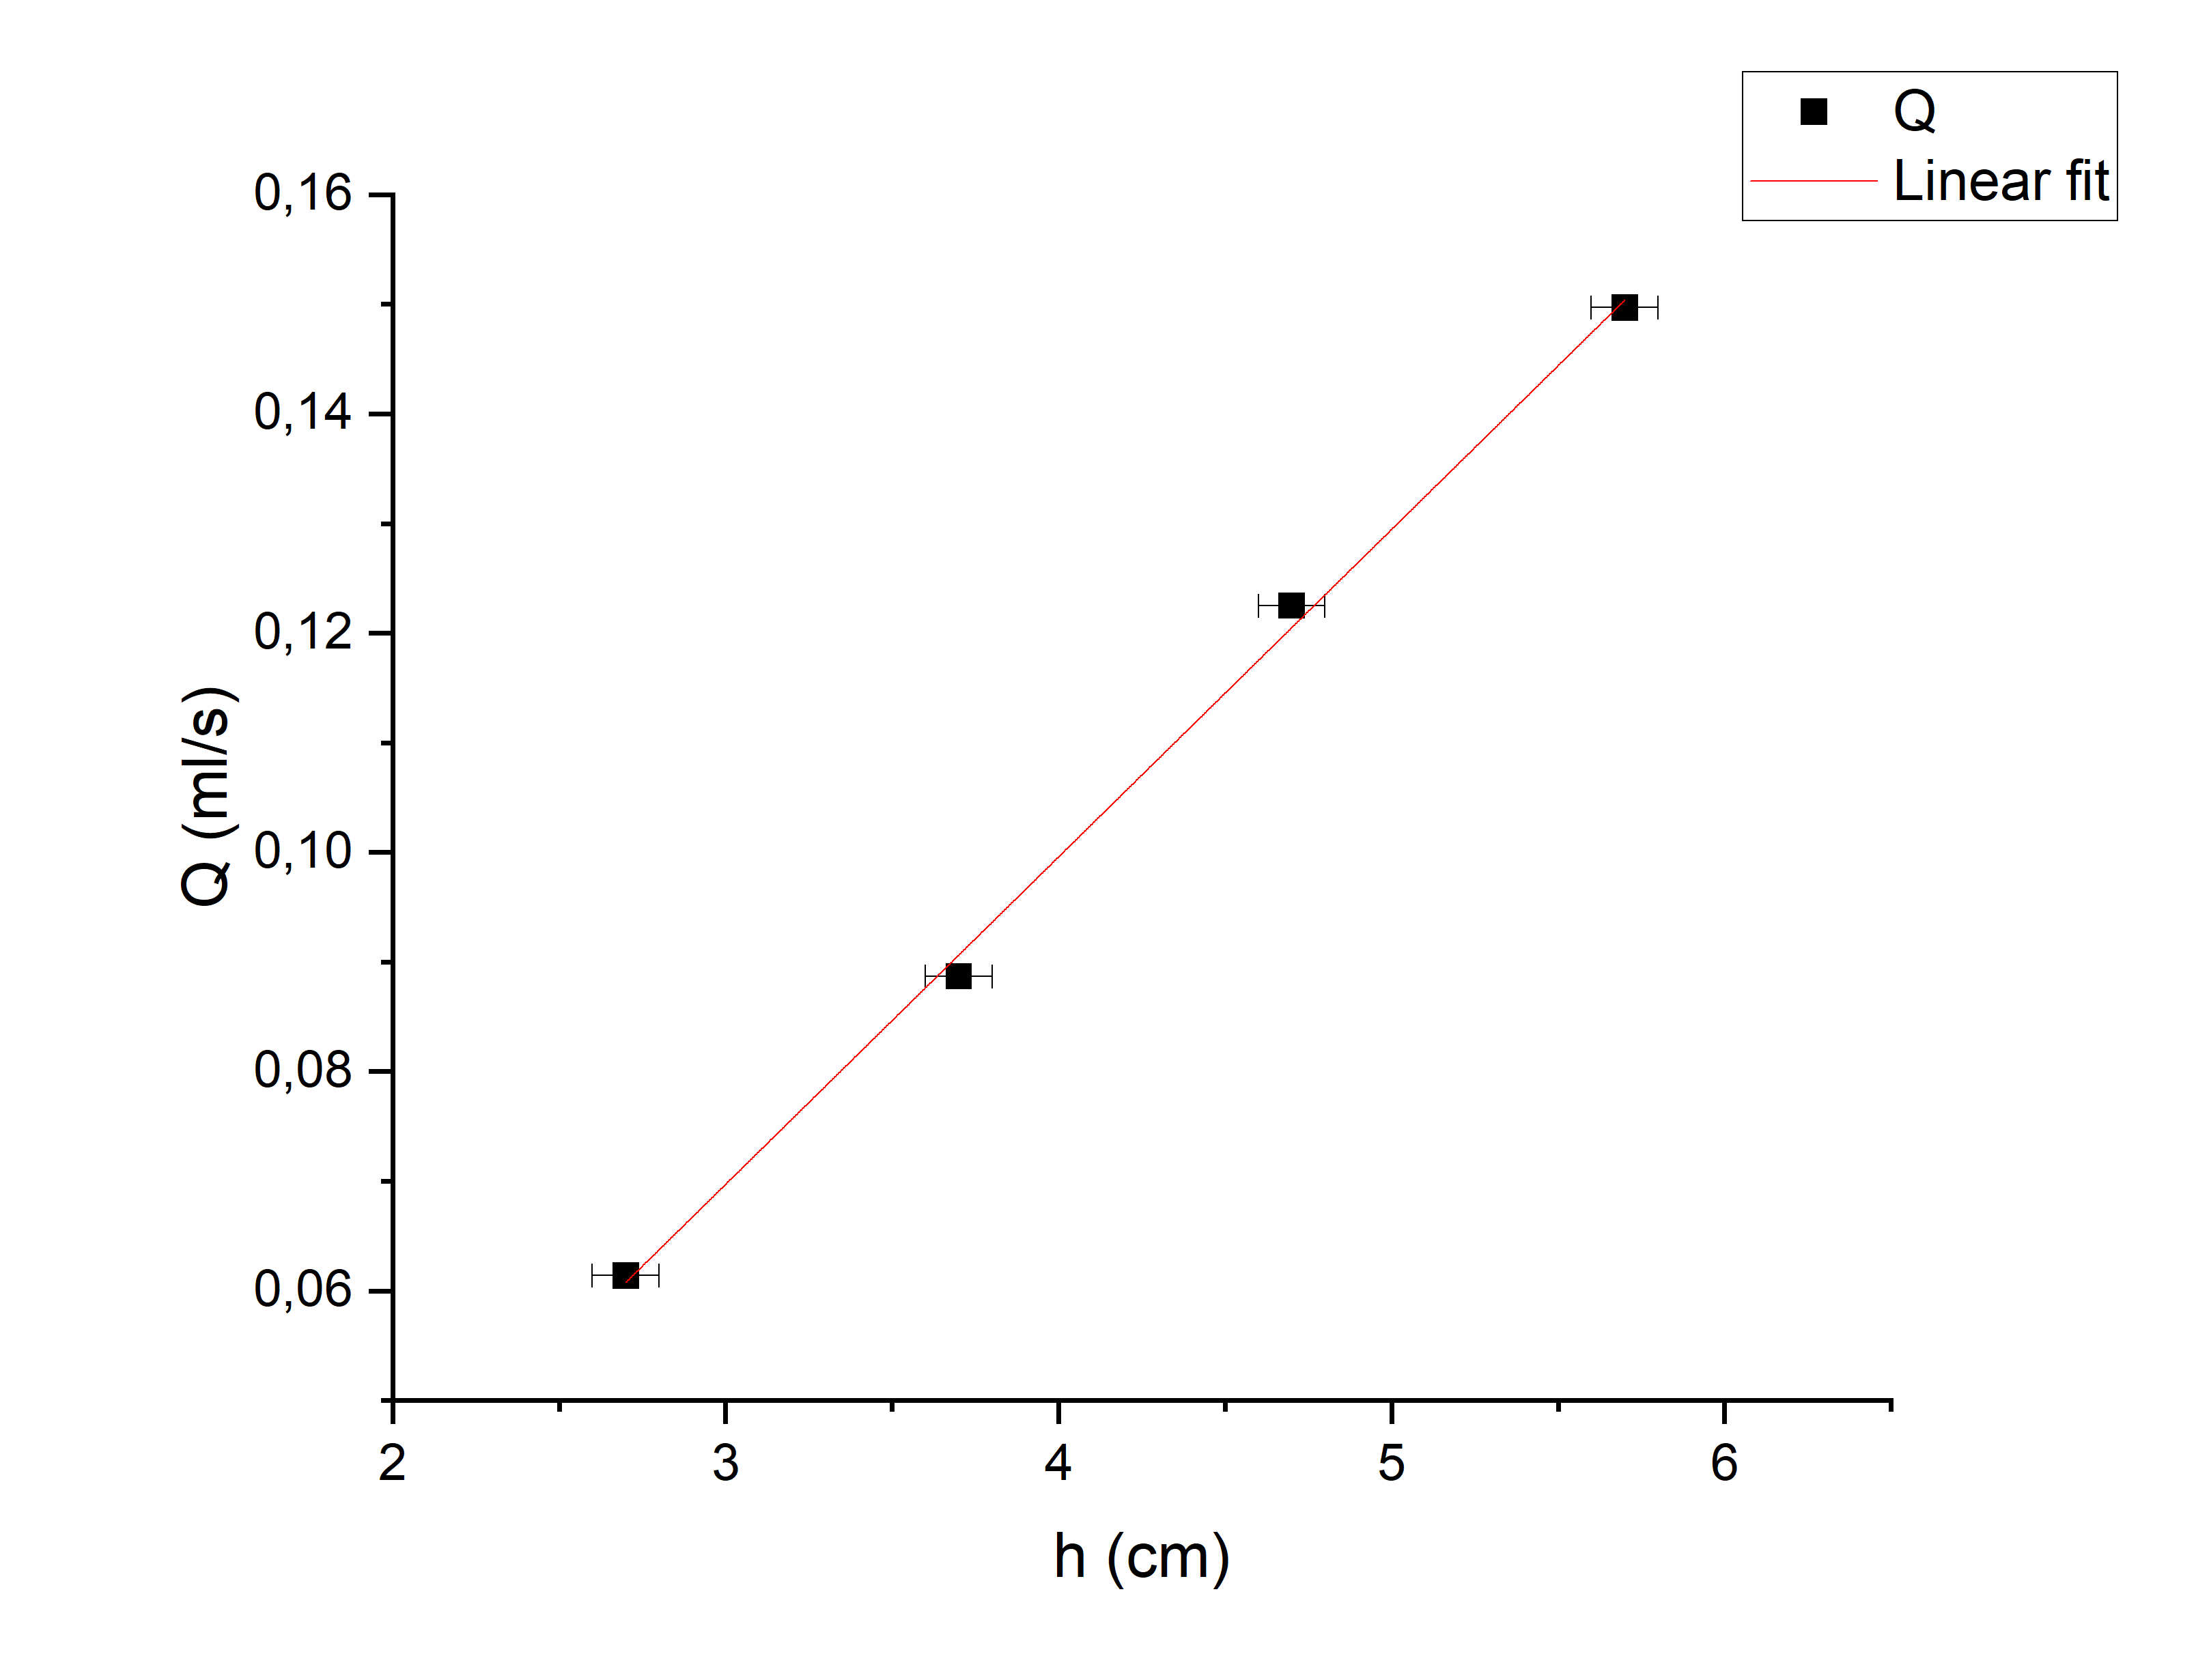
\includegraphics[scale=0.5]{PIC_2.png}
		\\\textbf{Рис. 2: } График зависимости $Q(h)$
	\end{center}

	%Страница 4
	
	\newpage
	
	\begin{flushleft}
		\footnotesize{Определение вязкости жидкости по скорости истечения через капилляр} \hspace{\fill} \footnotesize{4}
		\\[-0.3cm]\noindent\rule{\textwidth}{0.3pt}
	\end{flushleft}

	Методом линейной аппроксимации получаем:
	$$\gamma = (2.99 \pm 0.09) \cdot 10^{-2}\ \text{мл/см}\cdot\text{с}$$

	Теперь при помощи формулы Пуазейля выразим нужную нам вязкость:
	$$\eta = \sfrac{\pi R^4 \rho g}{8l\gamma} = (7.9 \pm 0.9)\cdot 10^{-4}\ \text{Па}\cdot\text{с}$$
	
	\subsection{Определение вязкости растворов глицерина вискозиметром Оствальда}
	
	\paragraph{Измерение времени протекания жидкостей}
	
	\begin{center}
		\begin{tabular}{|c|c|c|c|c|c|c|}
			\hline
			Раствор & \multicolumn{5}{|c|}{$\tau_i$, с} & $\overline{\tau}$, с \\\hline
			Вода & $6.24 \pm 0.20$ & $6.42 \pm 0.20$ & $6.45 \pm 0.20$ & $6.28 \pm 0.20$ & $6.30 \pm 0.20$ & $6.34 \pm 0.20$\\\hline
			Глицерин 10\% & $8.92 \pm 0.20$ & $8.81 \pm 0.20$ & $8.79 \pm 0.20$ & $8.71 \pm 0.20$ & $8.90 \pm 0.20$ & $8.86 \pm 0.20$
			\\\hline
			Глицерин 20\% & $11.86 \pm 0.20$ & $11.40 \pm 0.20$ & $11.44 \pm 0.20$ & $11.52 \pm 0.20$ & $11.88 \pm 0.20$ & $11.62 \pm 0.20$
			\\\hline
			Глицерин 30\% & $15.08 \pm 0.20$ & $15.90 \pm 0.20$ & $15.46 \pm 0.20$ & $15.38 \pm 0.20$ & $15.25 \pm 0.20$ & $15.41 \pm 0.20$
			\\\hline
		\end{tabular}
		\\\textbf{Табл. 3:} Измерение времени протекания
	\end{center}

	Теперь вспомним формулу для вязкости исследуемой жидкости:
	$$\eta_x = \eta_0 \sfrac{\rho_x t_x}{\rho_0 t_0}$$
	
	Необходимые данные и результаты вычислений оформим таблицей, при этом вязкость воды возьмем из предыдущей части эксперимента:
	\begin{center}
		\begin{tabular}{|c|c|c|c|}
			\hline
			Жидкость & $\rho_x$, г/см$^3$ & $t_x$, с & $\eta_x$, Па$\,\cdot\,$с
			\\\hline
			Вода & $1.000$ & $9.32 \pm 0.20$ & $(7.9 \pm 0.9) \cdot 10^{-4}$
			\\\hline
			Глицерин 10\% & 1.019 & $13.96 \pm 0.20$ & $(1.13 \pm 0.14) \cdot 10^{-3}$
			\\\hline
			Глицерин 20\% & 1.042 & $19.45 \pm 0.20$ & $(1.51 \pm 0.20) \cdot 10^{-3}$
			\\\hline
			Глицерин 30\% & 1.065 & $29.21 \pm 0.20$ & $(2.05 \pm 0.31) \cdot 10^{-3}$
			\\\hline
		\end{tabular}
	\end{center}
	
	\section{Выводы}
	
	В ходе работы определено значение вязкости воды $\eta = (7.9 \pm 0.9)\cdot 10^{-4}\ \text{Па}\cdot\text{с}$, что близко к табличному значению $\eta_0 = (8.9 \pm 0.9)\cdot 10^{-4}\ \text{Па}\cdot\text{с}$ в пределах двух величин стандартного отклонения.
	
	Также при помощи вискозиметра Оствальда определены вязкости нескольких растворов глицерина $\eta_{10\%} = (1.13 \pm 0.14)\cdot 10^{-3}\ \text{Па}\cdot\text{с}$, $\eta_{20\%} = (1.51 \pm 0.20)\cdot 10^{-3}\ \text{Па}\cdot\text{с}$, $\eta_{30\%} = (2.05 \pm 0.31)\cdot 10^{-3}\ \text{Па}\cdot\text{с}$, что также близко к табличным значениям в пределах двух стандартных отклонений.
\end{document}